\newpage
\section{Anti-aliasing filter}
The purpose of Anti-aliasing filter is to prevent aliasing of the signal, but also too suppress noise and get a better SNR. All sensor on the Rolling Road have an Anti-aliasing filter.  

\subsection{Design}

	
	\subsubsection{Calculation of low-pass filter to all the sensors.}
	
	In this section a Matlab script is used to make the best design for all the sensor.
	The script ADC\_lowpassFilter will automatic find the best components to realized the Anti-aliasing filters from E12 values, and will make sure that it will suppress the aliasing down to SNR of the ADC.
	
	
		
	\subsubsection*{Torque sensor}
	
	The following script will has been used to calculate the RC filter for the Torque sensor. But first some information is needed. The sample frequency, and how many bits it is using, what cut of frequency will be best. 
	The sample rate is 48000 and are using 12 bit. The cut of frequency is set to the max frequency what Rolling Road is gonna rotate if the AU2 is the test object. 
	
	\begin{lstlisting}
	ADC_fs=48000;
	ADC_N=12;
	fc=444/60; % RPM/60 = 1/s. Max rpm for Rolling Road then testning AU2 444RPM
	
	[R, C, fc_real, M]=ADC_lowpassFilter(ADC_fs, ADC_N, fc, [100*10^-12, 500*10^-9], 100*10^3, 66)
	
	T_AAF_Torque=tf(((1/(R*C))^M)/((s+1/(R*C))^M))
	
	figure;
	bode(T_AAF_Torque);
	legend('show');
	grid on;
	\end{lstlisting}
	
	The result from the script are:
	
	\begin{equation}
	\begin{split}
	R &= \SI{56}{\kilo\Omega}\\
	C &= \SI{390}{\nano\F}
	\end{split}
	\end{equation}
	
	And the transfer function is: 
	
	\begin{equation}
	T_{{AAF\_Torque}}(s) = \frac{45.79}{s+ 45.79}
	\end{equation}
	
	
	\begin{figure}[H]
		\centering
		\includegraphics [width=4in]{Hardware/Pictures/FilterAnalyse_01.eps}
		\caption{Bode plot of the Anti-aliasing filter for the Torque sensor}
		\label{fig:BODE_AAF_Torque}
	\end{figure}
	
	
	\subsubsection*{Power sensor}
	
	The signal of interest is the average value, because the PWM signal will be seen as noise signal, and must be filter out, also because els the sample rate have to be around 512 times bigger then PWM frequency.
	
	\begin{lstlisting}
	ADC_fs=52500;
	ADC_N=12;
	\end{lstlisting}
	
	calculate how much the PWM signal have to be suppress to meet the requirement of 0.1\% accuracy.
	
	\begin{lstlisting}
	Supress_dB=-20*log10(0.001)
	\end{lstlisting}


	
	The design will be build based on that the PWM frequency is greater then 2000Hz, and have to suppress the PWM signal 60dB too only getting a 0.1\% accuracy. This can be done with a 2. order low-pass filter 2 decades before 2000Hz this is 20Hz. The PWM signal will be suppress with 80dB.
	
	\begin{lstlisting}
	fc=20;
	
	[R, C, fc_real, M]=ADC_lowpassFilter(ADC_fs, ADC_N, fc, [100*10^-12, 500*10^-9], 100*10^3);
	
	T_AAF_power=tf(((1/(R*C))^M)/((s+1/(R*C))^M))
	
	figure;
	bode(T_AAF_power);
	legend('show');
	grid on;
	\end{lstlisting}

	The result from the script are. Note this is a 2 order low-pass filter:
	
	\begin{equation}
	\begin{split}
	R &= \SI{68}{\kilo\Omega}\\
	C &= \SI{120}{\nano\F}
	\end{split}
	\end{equation}
	
	And the transfer function is: 
	
	\begin{equation}
	T_{{AAF\_power}}(s) = \frac{15020}{{(s + 122.56)}^{2}}
	\end{equation}
	
	\begin{figure}[H]
		\centering
		\includegraphics [width=4in]{Hardware/Pictures/FilterAnalyse_02.eps}
		\caption{Bode plot of the Anti-aliasing filter for the power sensor}
		\label{fig:BODE_AAF_power}
	\end{figure}

\subsection{Implementation}

	Anti-aliasing filter will be realized in the implementation process. To implement the 2. order low-pass filter a buffer is needed, to realized the circuit. As a buffer the IC MCP6004 are used.
	
	\subsubsection*{Torque Sensor}
	
	\begin{figure}[H]
		\centering
		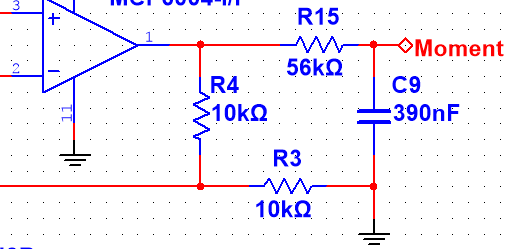
\includegraphics [width=4in]{Hardware/Pictures/AAF_moment.PNG}
		\caption{schematic of the Anti-aliasing filter for the torque sensor}
		\label{fig:schematic_AAF_Torque}
	\end{figure}
	
	There is not much too add to the torque sensor because it all ready has a buffer, and just a normal RC low-pass filter can be implement, as seen in \vref{fig:schematic_AAF_Torque} where R15 and C9 is the Anti-aliasing filter.
	
	
	\subsubsection*{Power sensor}

	\begin{figure}[H]
		\centering
		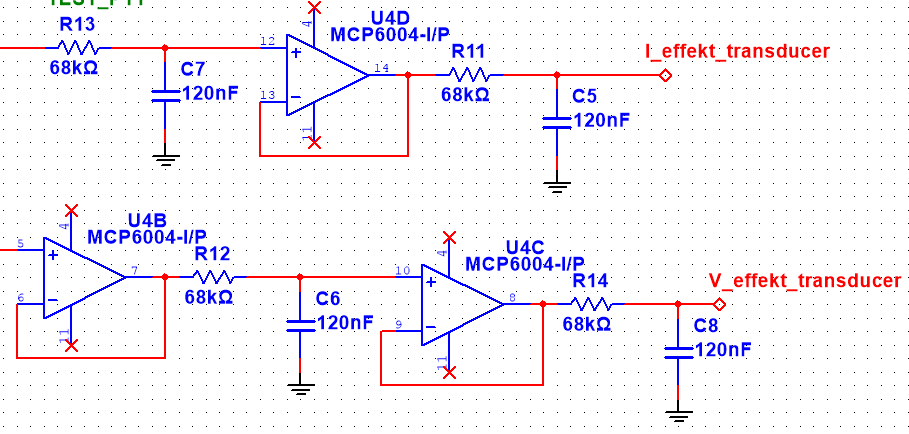
\includegraphics [width=4in]{Hardware/Pictures/AAF_effekt.PNG}
		\caption{schematic of the Anti-aliasing filter for the power sensor}
		\label{fig:schematic_AAF_power}
	\end{figure}
	
	The power sensor need a couple of buffer to make the 2. order low-pass filters. The reason what the I\_power\_sensor don't need a buffer in front of it is because the sensor all ready have a buffer inside of it.   

\subsection{Unity test}
Text \fxnote{Skal have udført en test når printet er færdigt!}